\documentclass{beamer}

\usepackage[utf8]{inputenc}
\usepackage[english]{babel}
\usepackage{graphicx}

\usetheme{Warsaw}

\title{Article Analysis}
\subtitle{A Robot Application for Marine Vessel Inspection}

\author{Mateus Santos de Cerqueira}
\institute{SENAI}
\date{\today}

\begin{document}
    \begin{frame}
        \titlepage
    \end{frame}
    
    \section{A Robot Application for Marine Vessel Inspection}
      
            \begin{frame}{INTRODUCTION}
                \begin{figure}[htb]
                    \centering
                    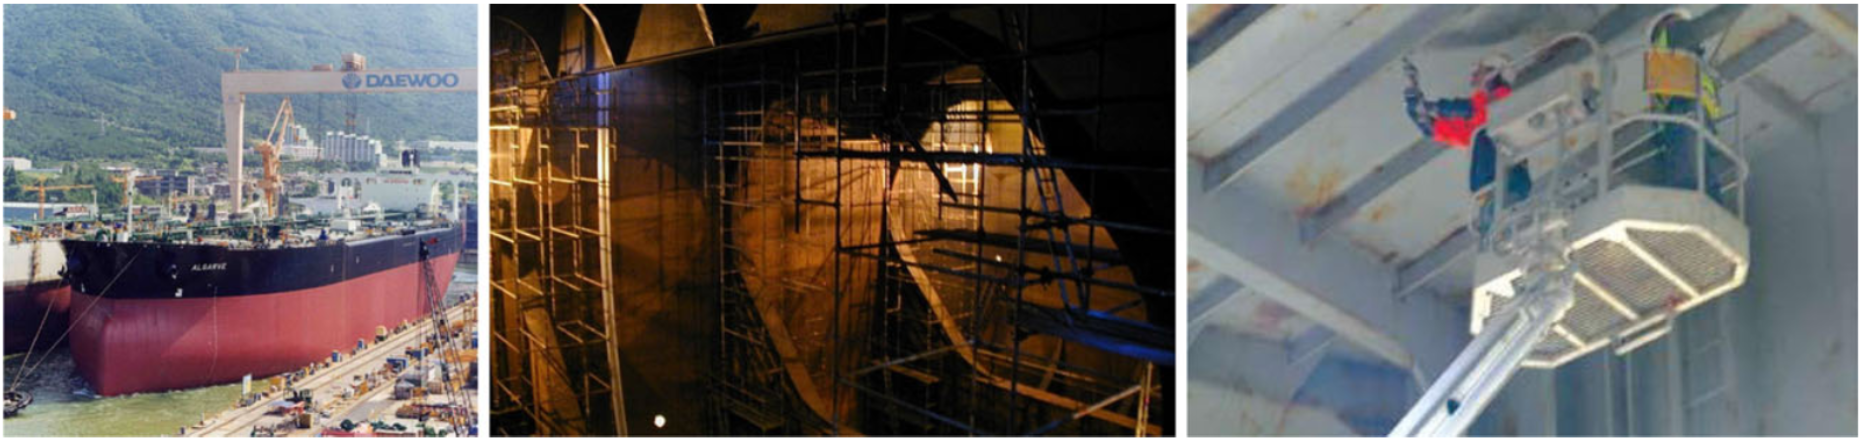
\includegraphics[scale=0.16]{figuras/traditional_inspection.png}                   
                    \caption{Traditional Inspection Methods}
                    \label{}                    
                \end{figure}
                    - Overview: \\
                    Traditional Inspection \\
                    MINOAS \\
                    Spatial Content Management System (SCMS)                
                           
            \end{frame}
            
        \subsection{REENGINEERED INSPECTION PROCEDURE}

            \begin{frame}{REENGINEERED INSPECTION PROCEDURE}
                \begin{figure}[htb]
                    \centering
                    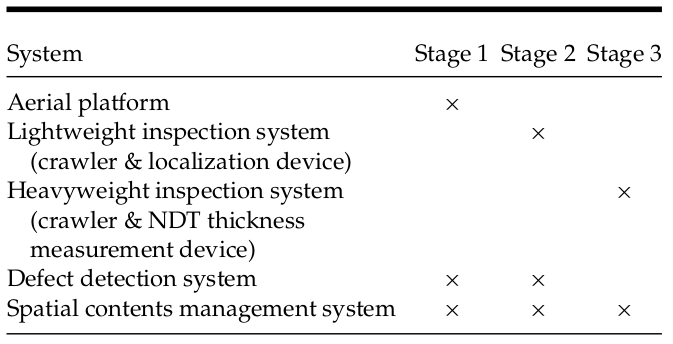
\includegraphics[scale=0.35]{figuras/inspection_stages}                   
                    \label{}
                    \caption{Relation Between Systems and Inspection Stages}
                \end{figure}


            \end{frame}

            \begin{frame}{MINOAS Inspecton Platforms}
                    \centering
                    Laser Scan \\
                    IMU \\
                    SLAM \\
                    Infrared or Ultrasound sensor \\ 
                    \pause                  
                    \begin{figure}[htb]
                        \centering
                        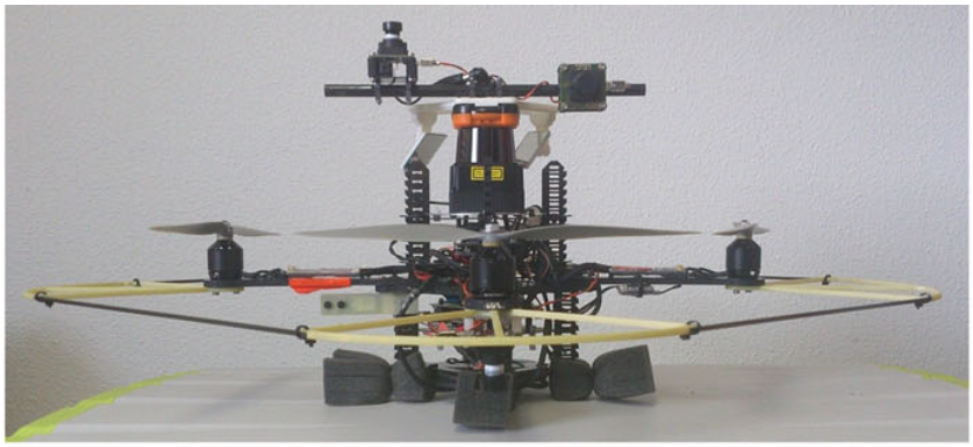
\includegraphics[scale=0.19]{figuras/platform_overview.png}                   
                        \label{}
                        \caption{Aerial Vehicle}
                    \end{figure}
            \end{frame}

        \subsection{AERIAL INSPECTION ROBOT}

            \begin{frame}{Aerial Inpection Robot}
                \centering
                Aerial Inspection Robot For Stage 1                
                    \begin{figure}[htb]
                        \centering
                        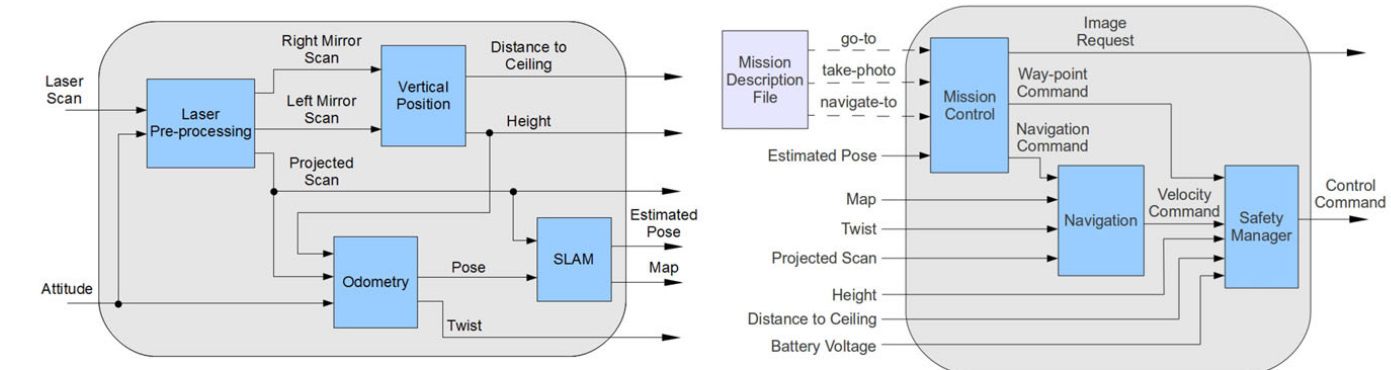
\includegraphics[scale=0.23]{figuras/self-localization.png}                   
                        \label{}
                        Self-Localization, Mapping and Mission Execution Modules
                    \end{figure} 
            \end{frame}

            \subsection{LIGHTWIGHT INSPECTION ROBOT}
            \begin{frame}{Lightweight Inspection Robot}
                \centering
                Lightweight Inspection Robot For Stage 2
                    \begin{figure}[htb]
                        \centering
                        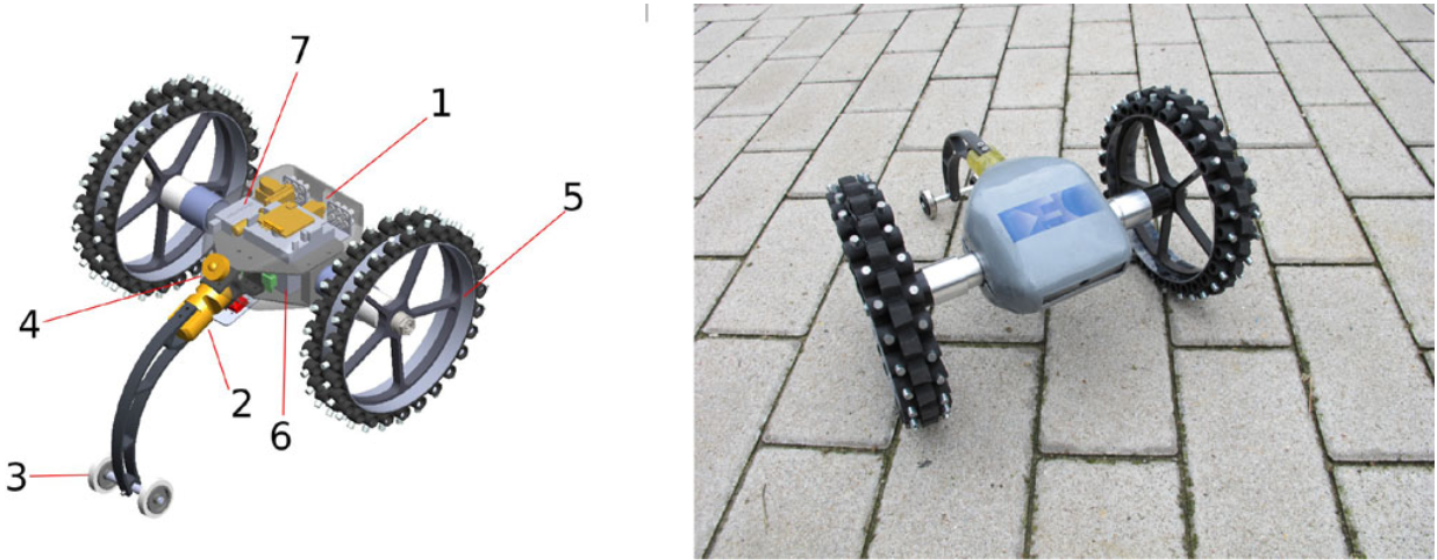
\includegraphics[scale=0.2]{figuras/lightweight_crawler.png}                   
                        \label{}
                        
                    \end{figure}                 
            \end{frame} 

            \begin{frame}{Lightweight Inspection Robot}
                \centering
                Lightweight Inspection Robot For Stage 2 
                    \begin{figure}[htb]
                        \centering
                        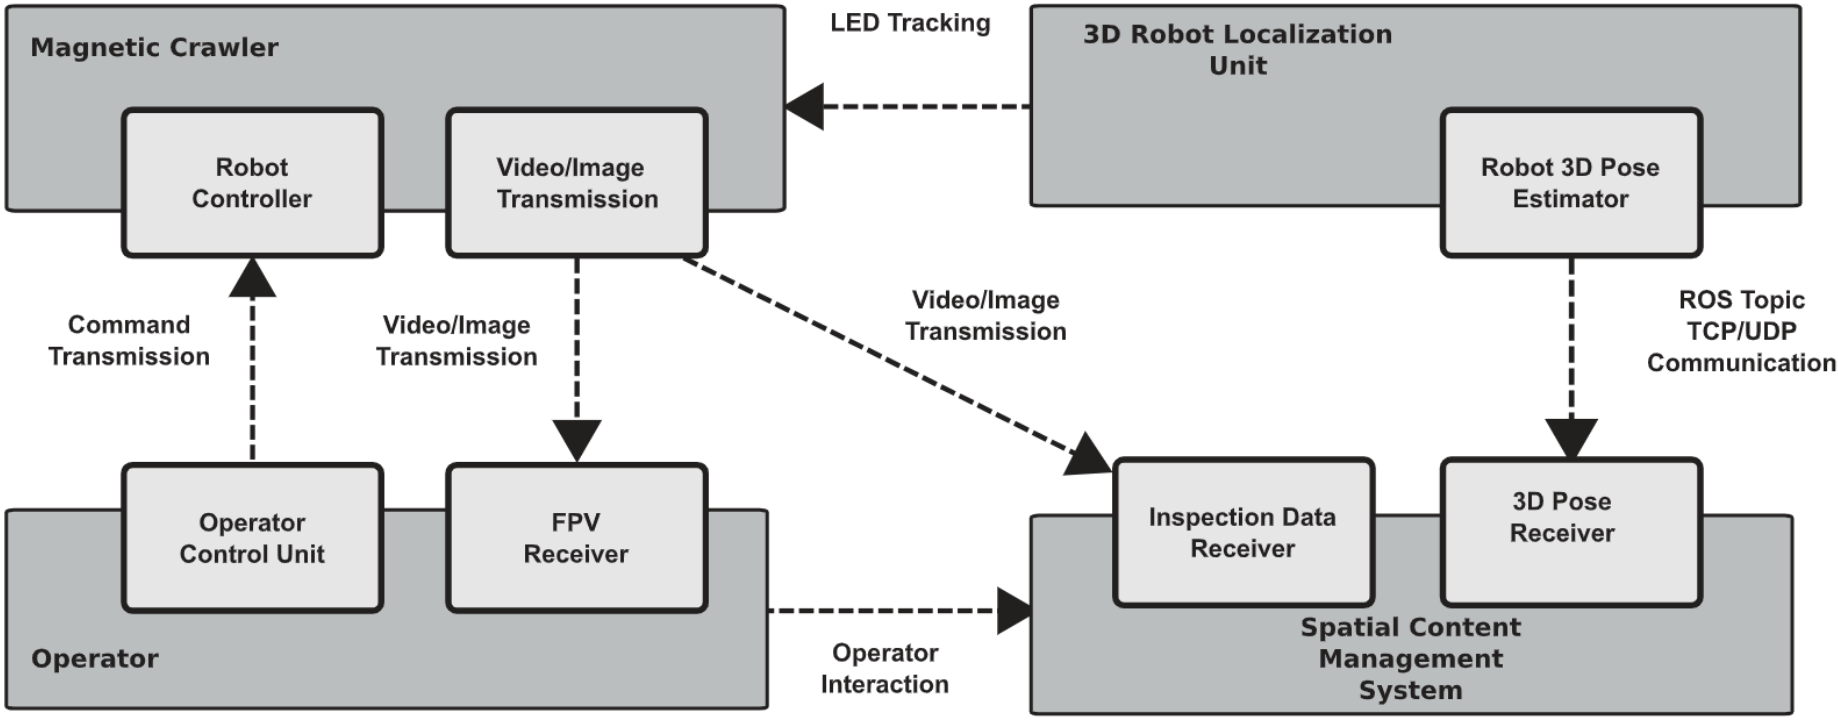
\includegraphics[scale=0.15]{figuras/overview_of_the_control_software_of_the_lightweight_system.png}                   
                        \label{}
                        Control Software of the Lightweight System
                    \end{figure} 
            \end{frame}        
            
        \subsection{HEAVYWEIGHT INSPECTION ROBOT}

            \begin{frame}{Heavyweight Inspection Robot}
                 
                \begin{figure}[htb]
                    \centering
                    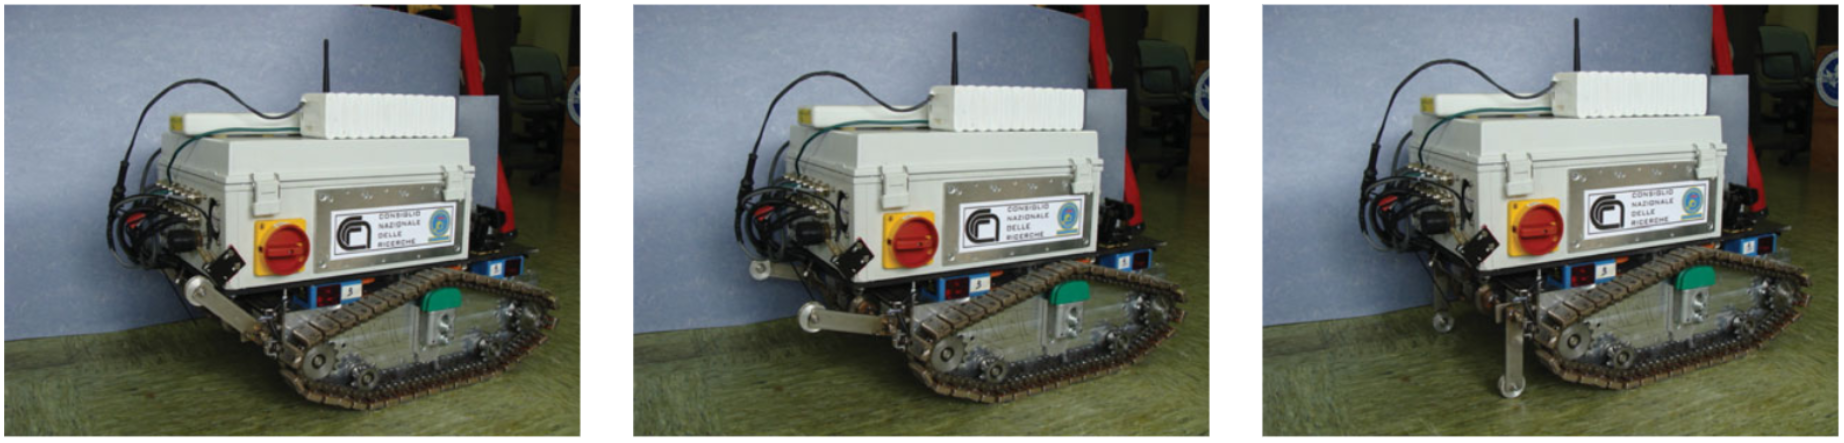
\includegraphics[scale=0.16]{figuras/MARC_rear_wheel_configurations.png}                   
                    \label{}
                    MARC Rear Wheel Configurations
                \end{figure}           
            \end{frame}            

        \subsection{A VISION-BASED SOLUTION FOR DEFECT DETECTION}
            \begin{frame}{A Vision-Based Solution for Defect Detection}
                - Corrosion Detection; \\
                    Roughness is measured \\
                    Color information \\
                - Crack Detection; \\
                    N x N pixel \\
                    M x M pixel \\ 
                \begin{figure}[htb]
                    \hfill 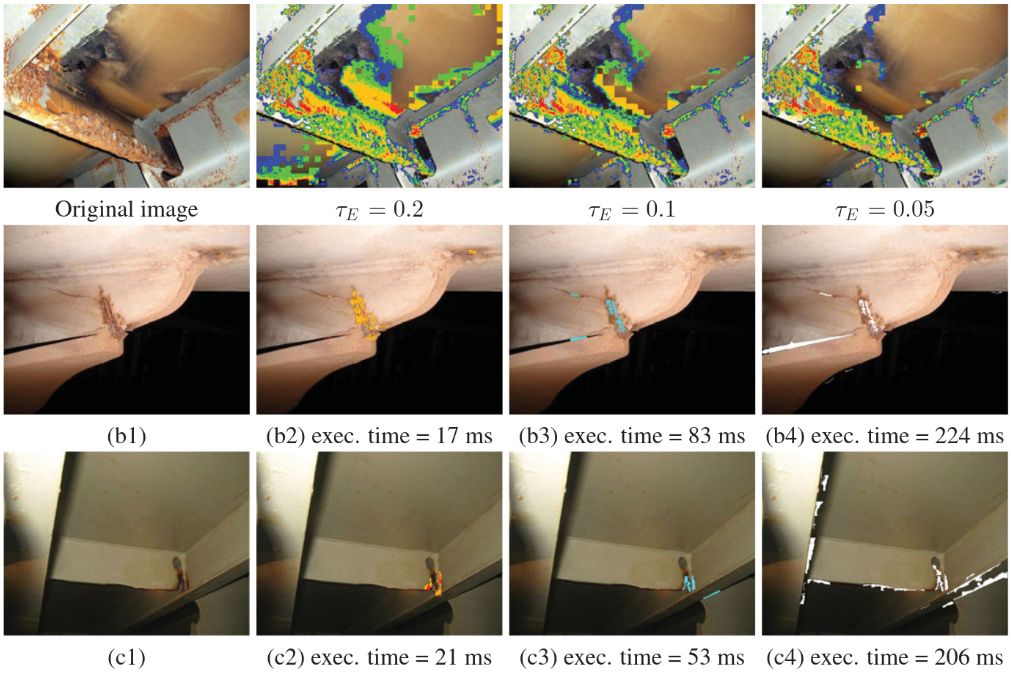
\includegraphics[scale=0.13]{figuras/corroded_aread_detected.png}                   
                    \label{}
                \end{figure}  
            \end{frame}        

        \subsection{SPATIAL CONTENT MANAGEMENT SYSTEM FOR ROBOT-ACQUIRED INSPECTION DATA}

            \begin{frame}{Spatial Content Management System for Robot-Acquired Inspection Data}
                \begin{figure}[htb]
                    \hfill 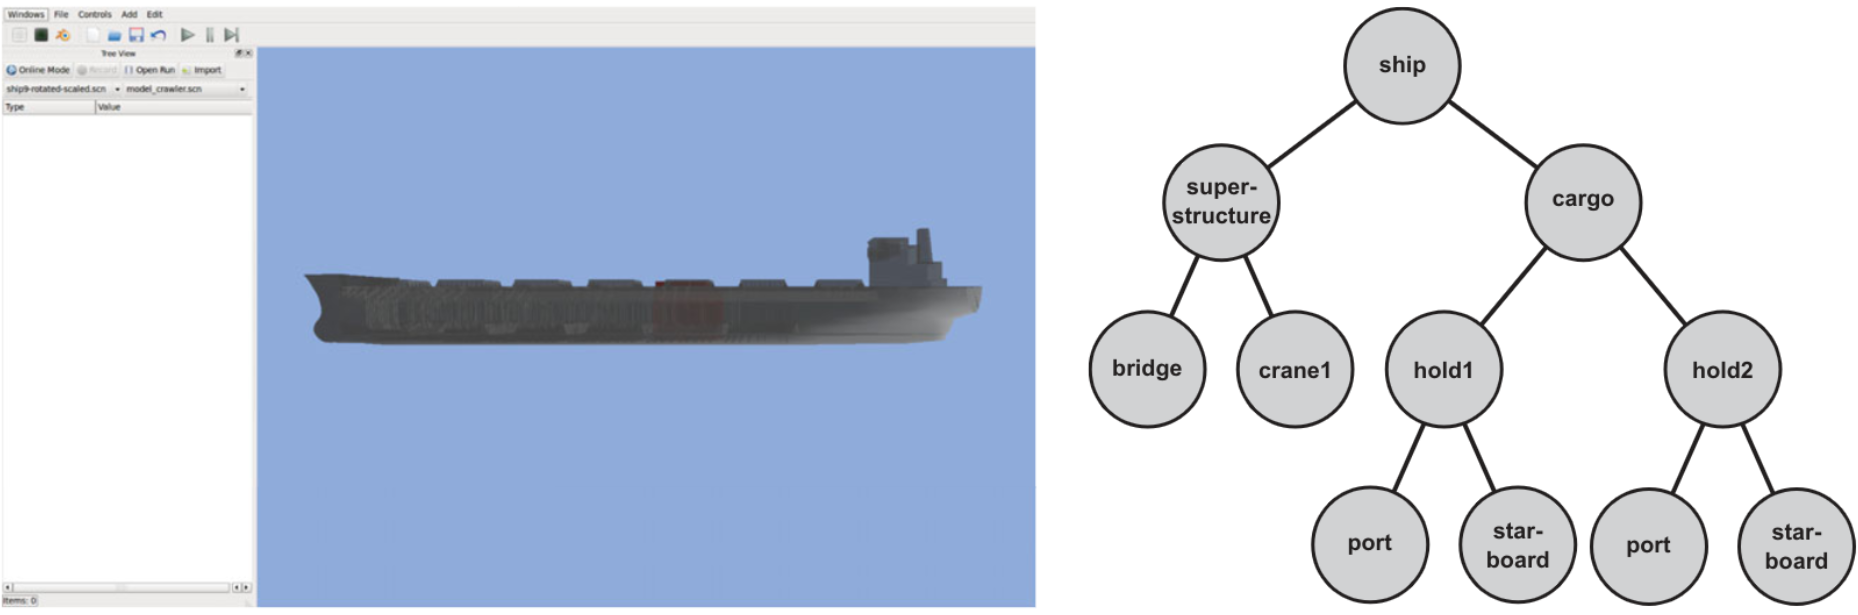
\includegraphics[scale=0.15]{figuras/the_spatial_content_management_system.png}                   
                    \label{}
                \end{figure}                 
                - SCMS Data; \\
                Collecting \\
                Sharing \\
                Displaying

            \end{frame}

        \subsection{SYSTEM PERFORMANCE EVALUATION}

            \begin{frame}{System Performance Evaluation}
                Micro-aerial vehicle (MAV) 
                \begin{figure}[htb]
                    \centering
                    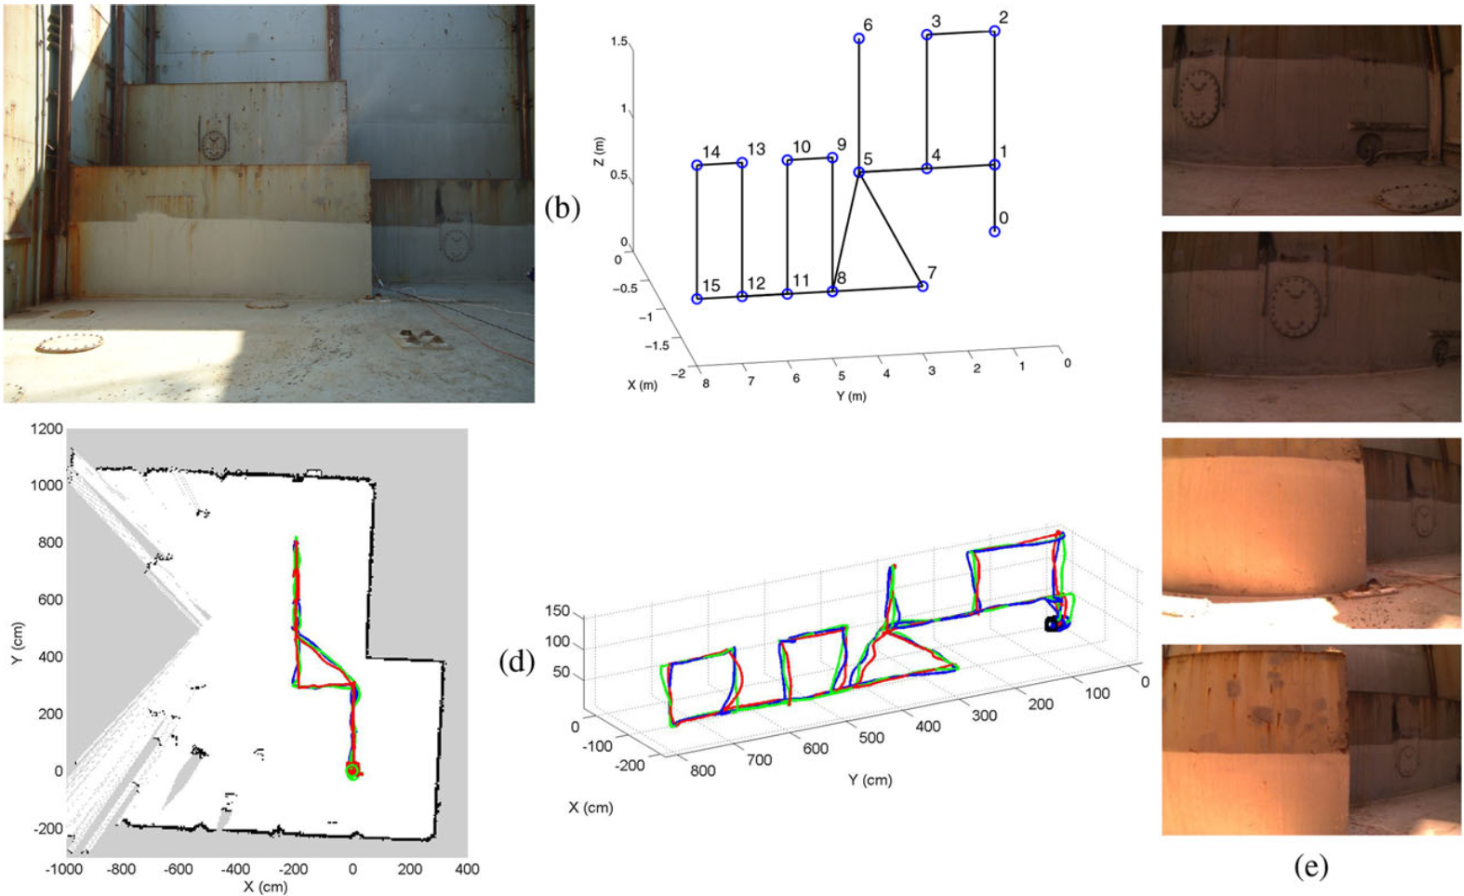
\includegraphics[scale=0.2]{figuras/MAV_results_in_autonomous_moode_from_the_second_field_trial.png}                   
                    \label{}
                \end{figure} 
            \end{frame}

            \begin{frame}{System Performance Evaluation}
                Lightweight Crawler  
                \begin{figure}[htb]
                    \centering
                    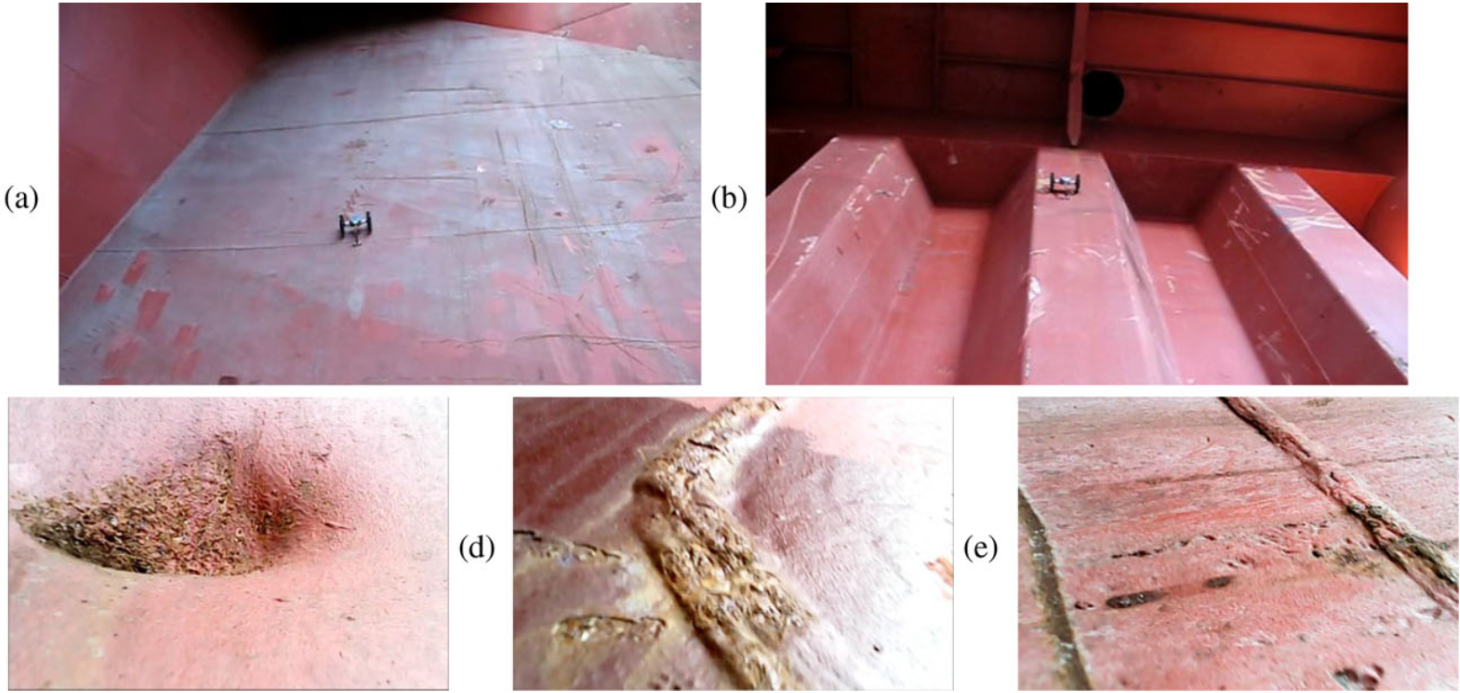
\includegraphics[scale=0.2]{figuras/frist_trial_for_the_lightweight_crawler.png}                   
                    \label{}
                \end{figure}         
            \end{frame}
            
            \begin{frame}{System Performance Evaluation}
                Heavyweight 
                \begin{figure}[htb]
                    \centering
                    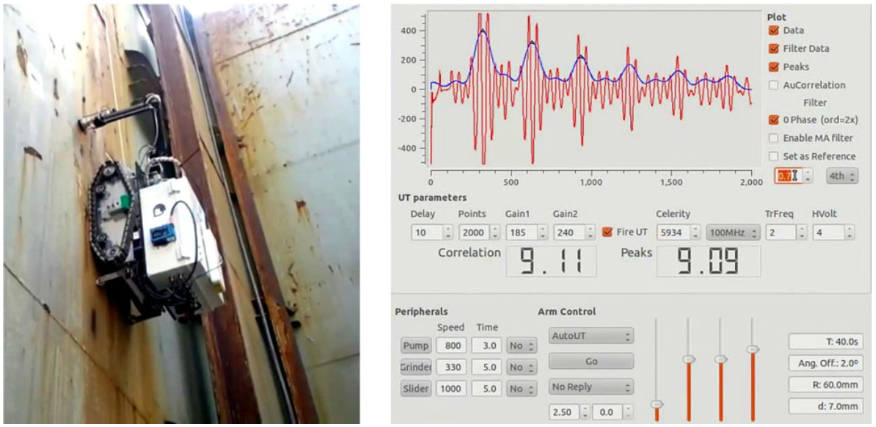
\includegraphics[scale=0.3]{figuras/MARC_on_a_vertical.png}                   
                    \label{}
                \end{figure}           
            \end{frame}
            
        \subsection{CONCLUSION AND FUTURE RESEARCH}
            \begin{frame}{Conclusion and Future Research}
                Vessel inspection \\
                Different locomotion capabilities \\
                Auxiliary systems \\
                Field trials \\
                SCMS
            \end{frame}
            
            \begin{frame}{Conclusion and Future Research}
                \centering Thanks           
            \end{frame}

\end{document}
